\chapter{Tinjauan Pustaka}

\section{Sistem untuk Permainan Musik Ekspresif}

Sistem komputer untuk permainan musik ekspresif (\textit{Computer Systems for Expressive Musical Performance} - CSEMP) adalah sistem yang dapat membangkitkan permainan musik yang ekspresif. Sebagai contoh, perangkat lunak \textit{typesetting} musik pada umumnya dapat memainkan musik secara "robotik". Sistem seperti ini bukan termasuk kategori sistem komputer untuk permainan musik ekspresif. Sistem komputer untuk permainan musik ekspresif mampu memainkan musik dengan sentuhan manusiawi. \parencite{miranda2010}

Ukuran yang digunakan untuk menentukan apakah suatu sistem komputer untuk permainan musik mampu memainkan musik dengan sentuhan manusiawi bermacam-macam, di antaranya kealamian \parencite{schubert2017test}, ekspresivitas, \textit{correctness}, dan kreativitas \parencite{miranda2010}. Kealamian atau \textit{humanness} merupakan ukuran seberapa pendengar manusia mampu membedakan permainan yang dibangkitkan sistem dari permainan manusia. Kealamian biasa diuji dengan tes buta pendengar atau tes Turing \parencite{schubert2017test}, baik dengan pendengar ahli maupun pendengar umum. Ukuran kinerja ekspresivitas dan \textit{correctness} dapat dilakuan dengan tes buta dengan pendengar ahli. Adapun kreativitas dapat diuji dengan menghitung banyaknya interpretasi berbeda yang dibangkitkan \parencite{miranda2010}. Umumnya, penelitian sistem permainan musik ekspresif saat ini berusaha meningkatkan kealamian.

Tujuan akhir dari sistem komputer untuk permainan musik ekspresif adalah membangkitkan suara yang memiliki gestur-gestur ekspresif dari not-not yang dideskripsikan dalam partitur. Masukan dari sistem ini adalah partitur. Partitur merupakan representasi dari sekumpulan not, yang mengindikasikan nada yang dimainkan beserta ritmenya. Contoh dari partitur tampak pada gambar \ref{humanmusicsheet} dan gambar \ref{midimusicsheet}.

\begin{figure}[h]
    \centering
    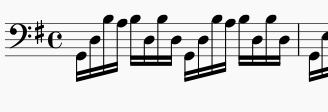
\includegraphics[width=0.8\textwidth]{resources/sheet-example-human.png}
    \caption{Contoh partitur dengan notasi not balok} \label{humanmusicsheet}
\end{figure}

\begin{figure}[h]
    \centering
    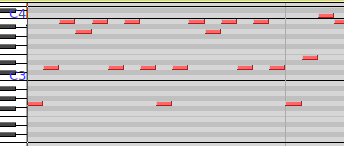
\includegraphics[width=0.8\textwidth]{resources/sheet-example-midi.png}
    \caption{Contoh partitur dalam representasi MIDI} \label{midimusicsheet}
\end{figure}

Keluaran dari sistem ini adalah suara yang di dalamnya terkandung gestur-gestur ekspresif. Contoh representasi suara terlihat pada gambar \ref{waveformexample} dan gambar \ref{spectogramexample}. Gambar \ref{waveformexample} adalah gambaran suara dalam bentuk \textit{waveform}, yang dapat diubah menjadi spektogram pada gambar \ref{spectogramexample}. Gestur ekspresif implisit terkandung dalam suara yang dihasilkan, berupa distorsi waktu, distorsi \textit{pitch}, variasi dinamika, variasi timbre, dan fitur-fitur suara lainnya.

Dalam bentuk spektogram, atau fitur akustik lainnya, ataupun dalam bentuk representasi gestur ekspresi, koefisien korelasi kepada referensi pemain manusia juga dapat digunakan sebagai salah satu ukuran kinerja. Koefisien korelasi menunjukkan keberhasilan sistem membangkitkan ekspresi musik yang sesuai dengan pola-pola ekspresi musik manusia. \parencite{schubert2017test} \parencite{lindemann2007rpm}

\begin{figure}[h]
    \centering
    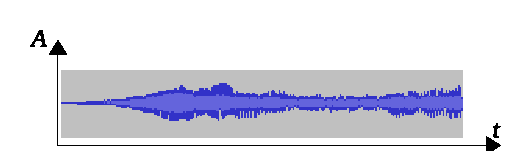
\includegraphics[width=0.8\textwidth]{resources/waveform-example.eps}
    \caption{Contoh representasi bentuk gelombang dari suara keluaran} \label{waveformexample}
\end{figure}

\begin{figure}[h]
    \centering
    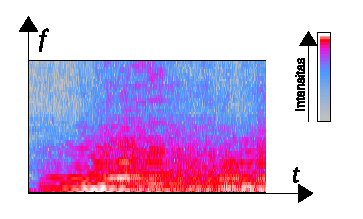
\includegraphics[width=0.8\textwidth]{resources/spectogram-example.eps}
    \caption{Contoh representasi spektogram dari suara keluaran} \label{spectogramexample}
\end{figure}

Komponen sistem ini dapat dibagi menjadi sistem perencana gestur dan pembangkit suara \parencite{Thippur2013ProbabilisticMO} seperti pada gambar \ref{thippurcomponents}. Keluaran dari sistem perencana gestur adalah rencana gestur ekspresif seperti keras-lemah suara, deskripsi timbre, deskripsi tempo, dan deskripsi teknik permainan spesifik alat musik. Komponen-komponen sistem ini dapat pula dipisahkan menjadi sistem perencana ekspresi, perencana gestur, dan pembangkit suara \parencite{yu2017bowing} seperti terlihat pada gambar \ref{yucomponents}. Perencana ekspresi bertugas membaca partitur dan menentukan rencana ekspresi dalam permainan tersebut. Contoh rencana ekspresi adalah \textit{espressivo} (ekspresif), \textit{scherzando} (melawak), \textit{tranquillo} (tenteram), dan sebagainya \parencite{yang2016synthesis}.

Suara yang dihasilkan dalam suatu permainan dipengaruhi oleh rencana gestur yang dieksekusi. Representasi rencana gestur dan informasi yang terkandung di dalamnya bergantung kepada jenis alat musik dan desain sistem. Spesifikasi energi tiap not, yang berhubungan dengan keras lemahnya not, lalu kepada alur perubahan dinamika sepanjang lagu, umum digunakan pada banyak alat musik. Spesifikasi energi di dalam not dan perubahannya sepanjang not mungkin hanya relevan untuk alat musik dengan eksitasi kontinu seperti alat gesek, alat tiup, dan nyanyian. Pada alat gesek, spesifikasi energi dan pilihan warna suara mungkin saja digantikan dengan spesifikasi cara menggesek (\textit{bowing}). Posisi \textit{bowing} dapat diubah, baik dari jarak dengan \textit{bridge} maupun pada bagian \textit{bow} mana senar tertempel. Begitu pula kecepatan dan tekanan \textit{bowing} dapat berpengaruh kepada \textit{timbre} dan dinamika. \parencite{yu2017bowing} Contoh gestur lainnya adalah \textit{vibrato}: naik turunnya \textit{pitch} (tinggi rendahnya frekuensi formant utama/\textit{f0}) dalam alat musik gesek atau naik turunnya amplitudo secara periodik dalam satu not. Gestur \textit{vibrato} mungkin saja sudah implisit terkandung dalam rencana realisasi \textit{pitch}. Dalam desain representasi rencana gestur, satu jenis gestur mungkin tidak digunakan karena sudah terkandung secara implisit dalam jenis gestur lain, data lain, atau bahkan mungkin pula diabaikan.

Dalam pembangunan CSEMP dan komponennya, pembagian ini tidak mutlak. Selain sistem yang membuat rencana-rencana ekspresi dan gestur terlebih dahulu sebelum dieksekusi menjadi suara, terdapat pula sistem yang langsung membangkitkan suara dari partitur tanpa adanya keluaran antara.

\begin{figure}[h]
    \centering
    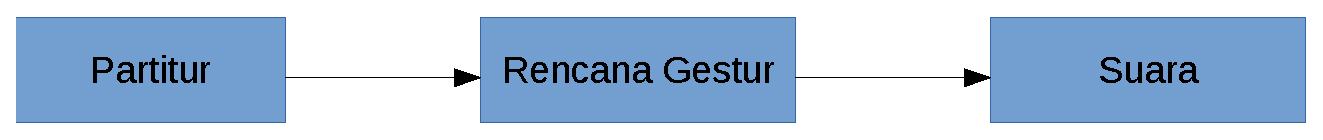
\includegraphics[width=0.8\textwidth]{resources/CSEMP-Components-Thippur.eps}
    \caption{Komponen-komponen CSEMP berdasarkan \citet{Thippur2013ProbabilisticMO}} \label{thippurcomponents}
\end{figure}

\begin{figure}[h]
    \centering
    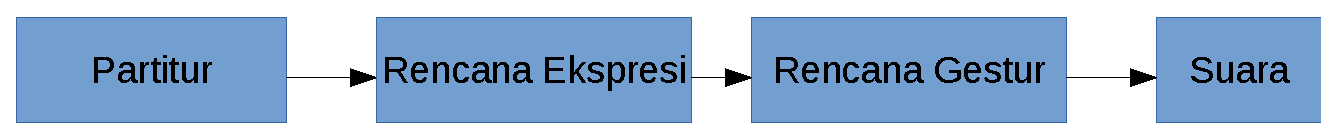
\includegraphics[width=0.8\textwidth]{resources/CSEMP-Components-Yu.eps}
    \caption{Komponen-komponen CSEMP berdasarkan \citet{yu2017bowing}}\label{yucomponents}
\end{figure}

\textit{Scope} dari penelitian-penelitian sebelumnya bermacam-macam. Terdapat sistem permainan music ekspresif yang bersifat \textit{end-to-end}, yaitu membangkitkan suara ekspresif dari masukan partitur. Penelitian bonada \parencite{bonada2017singing} membangkitkan suara vokal ekspresif dari partitur. Meski jangkauan konteks temporal yang dipertimbangkan dalam sistem Bonada hanya meliputi waktu yang dekat (dengan medan reseptif 100ms jaringan syaraf tiruan dengan konvousi terdilasi), suara yang dibangkitkan memiliki ekspresi dengan taraf tertentu. Suara yang dibangkitkan dengan sistem Bonada telah diujikan pula kepada pendengar manusia, meski belum mencapai taraf kealamian seperti pemain manusia.

Sistem lainnya yang telah mampu membangkitkan suara dari partitur saja (\textit{end-to-end}) adalah CaRo \parencite{canazza2015}. Untuk memainkan partitur dan membangkitkan suara, CaRo mengirimkan sinyal perintah permainan kepada mesin piano akustik. Dalam uji pendengar manusia \parencite{schubert2017test}, dibuktikan bahwa permainan CaRo tidak dapat dibedakan dari permainan manusia oleh pendengar manusia.

Terdapat penelitian lain yang hanya melingkupi sistem perencanaan gestur saja. Salah satunya adalah sistem perencanaan gestur untuk alat musik dengan eksitasi diskrit \parencite{miranda2010}. Ukuran kinerja dari sistem seperti ini hanya berupa akurasi dari data gestur ekspresi.

Terdapat penelitian lain yang hanya melingkupi sintesis suara saja. Nsynth \parencite{nsynth2017} mampu membangkitkan alat musik secara umum. Namun, suara yang dihasilkan hanya berupa suara satu not.

\section{Sistem Permainan dan Sintesis Musik Ekspresif Alat Musik Gesek}

Belum ada sistem permainan dan sintesis ekspresif untuk alat musik gesek yang mampu membangkitkan dari masukan partitur saja menjadi suara ekspresif. Telah ada penelitian-penelitian yang mengajukan komponen dari CSEMP untuk alat musik gesek.

Telah ada teknik sintesis yang mampu menghasilkan suara berbagai instrumen - termasuk alat musik gesek - dengan frasa yang natural, yaitu teknik \textit{Reconstructive Phrase Modeling} \parencite{lindemann2007rpm}. Input dari sistem ini adalah partitur dan gestur ekspresif. Gestur ekspresif yang menjadi masukan terdiri dari kontrol tiap not dan kontrol kontinu. Kontrol tiap not terdiri dari \textit{pitch} dan intensitas not. Kontrol kontinu terdiri dari intensitas \textit{vibrato}, tingkat keras instrumen, timbre, dan \textit{pitch-bend}. Keluaran dari sistem ini adalah prediksi harmonik, yang kemudian dapat langsung digunakan untuk sintesis suara.

Meski sudah dapat menghasilkan suara, penelitian \citet{lindemann2007rpm} masih membutuhkan masukan gestur ekspresif yang memiliki beberapa  masalah. Masalah pertama adalah format dari deskripsi gestur tidak didasarkan pada cara permainan alat musik gesek melainkan \textit{keyboard}. Masalah kedua, yang juga disebabkan masalah pertama, adalah besarnya kemungkinan kesalahan masukan gestur ekspresi baik pada data latih maupun pada pengujian/penggunaan sistem. Masalah lainnya adalah tidak tidak fleksibelnya keluaran yang dihasilkan, karena teknik \textit{Reconstructive Phrase Modeling} mencocokkan masukan dengan basis data frasa dan memainkan serupa dengan frasa yang telah ada di basis data.

Terdapat sistem lain yang membangkitkan \textit{waveform} secara langsung tanpa melalui prediksi harmonik. Nsynth \parencite{nsynth2017} mampu menghasilkan satu not saja. Meski suara yang dihasilkan diklaim berupa suara natural, namun karena yang dibangkitkan hanya satu not, sistem ini belum mampu membangkitkan suara musik dari partitur yang mengandung satu lagu lebih dari satu not secara ekspresif. Suara yang dihasilkan akan memiliki gestur ekspresi yang sama untuk setiap not.

Terdapat sistem serupa menghasilkan suara yang tidak mempertimbangkan konteks not \parencite{yang2016synthesis}. Namun, sistem ini mampu mempertimbangkan \textit{term} ekspresi musik yang diberikan sebagai input. Sistem ini mampu menghasilkan suara dengan manipulasi durasi, vibrato, dan dinamika. Pengujiannya dilakukan dengan kemiripan visual spektogram. Kekurangannya adalah di satu karya dengan satu ekspresi musik, not yang memiliki panjang sama akan diberi gestur yang sama.

Beberapa sistem lain hanya memberikan perencanaan gestur alat musik gesek. Terdapat sistem yang mampu memberikan rencana gestur untuk kuartet alat musik gesek. \parencite{marchini2014quartet} Sistem ini mampu membangkitkan rencana gestur berupa tingkat keras suara, kecepatan \textit{bow}, jangkauan \textit{vibrato}, dan perpanjangan not. Pengujian dalam penelitian tersebut hanya dilakukan terhadap satu kutipan karya yang sama dengan data latih dengan ukuran kinerja koefisien korelasi.

Terdapat sistem perencanaan gestur lainnya untuk alat musik violin dan viola \parencite{yu2017bowing}, namun gestur yang dihasilkan hanya berupa posisi \textit{bowing}. Sistem tersebut mampu menerima masukan partitur dan menghasilkan posisi \textit{bowing} tiap not seperenambelasan. Pengujian sistem ini telah dilakukan hanya terhadap satu kutipan karya dengan data latih berupa kutipan karya lain. Kinerja sistem ini diukur dengan koefisien korelasi dan akurasi.

Meski terdapat komponen-komponen CSEMP alat musik gesek, terdapat masalah dalam penggabungan komponen sistem yang telah ada. Pertama, output dari sistem yang telah ada bisa jadi tidak lengkap \parencite{yu2017bowing}. Kedua, sistem yang ada tidak kompatibel untuk langsung digabungkan. Input untuk sistem sintesis yang telah ada \parencite{lindemann2007rpm} menerima masukan dari pemain \textit{keyboard}. Sistem sintesis tersebut tidak mendukung masukan kecepatan \textit{bow} \parencite{marchini2014quartet}\parencite{yu2017bowing} dan posisi \textit{bow}\parencite{yu2017bowing}. Gestur \textit{vibrato} dalam alat musik gesek terdiri dari jangkauan dan kerapatan, sementara dalam masukan \textit{keyboard} disederhanakan menjadi intensitas saja.

Terdapat sebuah \textit{framework} CSEMP alat musik gesek untuk pembangkitan suara dari partitur non-expresif \parencite{perez2015} menggunakan pemodelan instrumen, pemain dan akustik. Namun, sistem ini hanya berupa \textit{framework} umum yang perlu didetilkan kembali. Selain itu, pemisahan pemodelan ini meniscayakan kebutuhan anotasi gestur secara manual.

\section{Sintesis Parametrik Neural} \label{literature-neural-parametric}

\citet{bonada2017singing} mengajukan sebuah teknik untuk sintesis suara nyanyian ekspresif. Suara nyanyian dibangkitkan dengan sebuah \textit{vocoder} dengan parameter-parameter \textit{timing} fonetik, \textit{timbre}, dan \textit{pitch}. Parameter-parameter ini dibangkitkan dengan model \textit{timing} fonetik, model \textit{timbre}, dan model \textit{pitch} yang dilatih dengan data latih partitur non ekspresif dan suara nyanyian ekspresif. Arsitektur sistem ini tampak pada gambar \ref{fig-system-overview-bonada}. Pemisahan model ini dilakukan untuk mengatasi lambatnya pembangkitan 	extit{waveform} secara langsung menggunakan satu model tunggal pada WaveNet\parencite{Oord2016WaveNetAG}. Pemisahan model memungkinkan pembangkitan parameter akustik per \textit{frame} yang \textit{rate}-nya jauh lebih sedikit daripada \textit{sample rate} pada \textit{waveform}.

\begin{figure}[h]
    \centering
    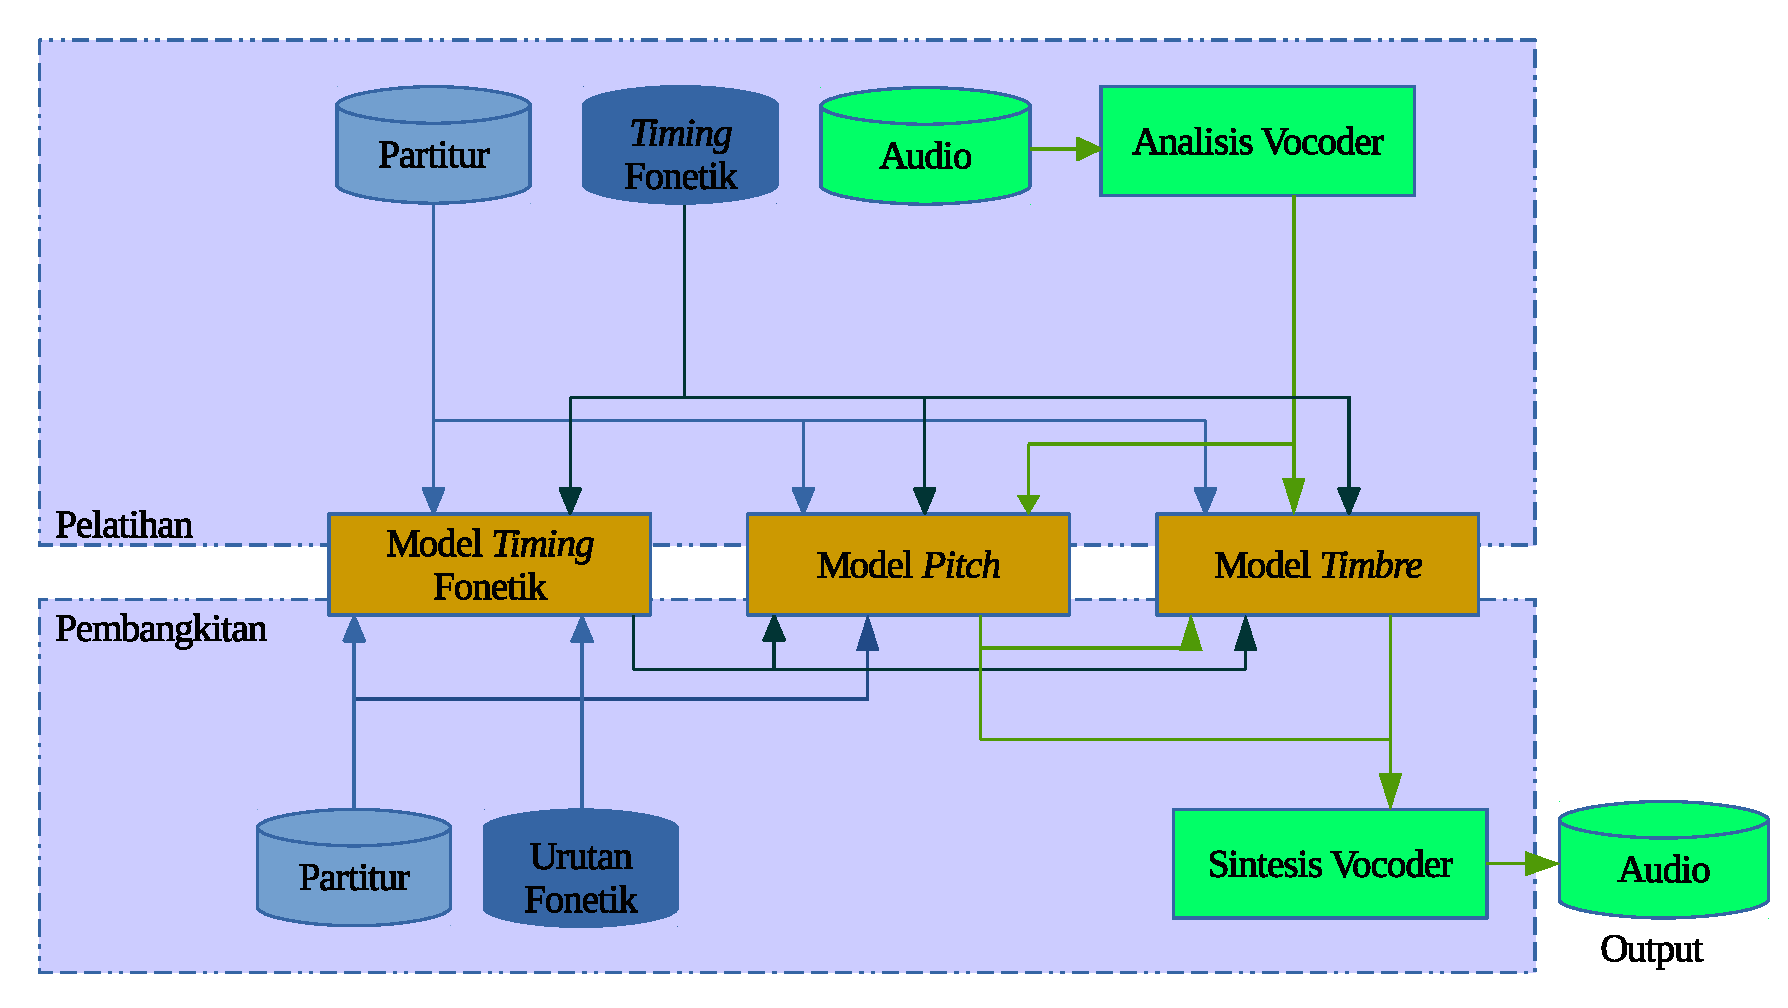
\includegraphics[width=0.8\textwidth]{resources/system-overview-bonada.eps}
    \caption{Arsitektur sistem sintesis parametrik neural untuk nyanyian \parencite{bonada2017singing}}\label{fig-system-overview-bonada}
\end{figure}

Dalam sistem ini, terdapat tiga model, yang menghasilkan parameter-parameter yang kemudian digunakan \textit{vocoder} untuk menghasilkan suara nyanyian ekspresif. Model-model ini dilatih menggunakan data latih berupa partitur, label \textit{timing} fonetik, dan rekaman penyanyi profesional yang bersesuaian. Rekaman penyanyi dianalisis dengan vocoder untuk mendapatkan representasi \textit{pitch} dan \textit{timbre}. Masukan dan keluaran tiap model tercantum dalam tabel \ref{tab-models-in-out-bonada}

\begin{table}[h]
	\centering
    \caption{Masukan dan Keluaran Tiap Model dalam Sistem Sintesis Parametrik Neural Suara Nyanyian \parencite{bonada2017singing}}\label{tab-models-in-out-bonada}
	\begin{tabular}{ |c|c|c| } 
	 \hline
	 Model & Masukan & Keluaran \\
	 \hline 
	 Model \textit{timing} & partitur & \textit{timing} (terdistorsi) not \\ 
	 fonetik  & urutan fonetik & \textit{timing} fonetik \\ 
	 \hline
	 Model \textit{pitch} & partitur & F0 \\ 
	  & \textit{timing} (terdistorsi) not  & \\ 
	 \hline
	 Model \textit{timbre} &  \textit{timing} fonetik\&not & V/UV \\ 
	  & F0 & Komponen harmonik\\ 
	  &   & Komponen aperiodisitas\\ 
	 \hline
	\end{tabular}
\end{table}

Untuk model \textit{timing} not, digunakan jaringan syaraf tiruan \textit{feedforward} dengan fitur kontekstual untuk tiap not dalam partitur. Untuk model \textit{durasi} fonem, digunakan jaringan syaraf tiruan konvolusional. \parencite{bonada2017singing} Untuk model \textit{pitch} dan model \textit{timbre}, digunakan jaringan syaraf tiruan dengan arsitektur yang didasarkan kepada WaveNet \parencite{Oord2016WaveNetAG}, yang tampak pada gambar \ref{fig-network-architecture-bonada}. \parencite{bonada2017singing}

\begin{figure}[h]
    \centering
    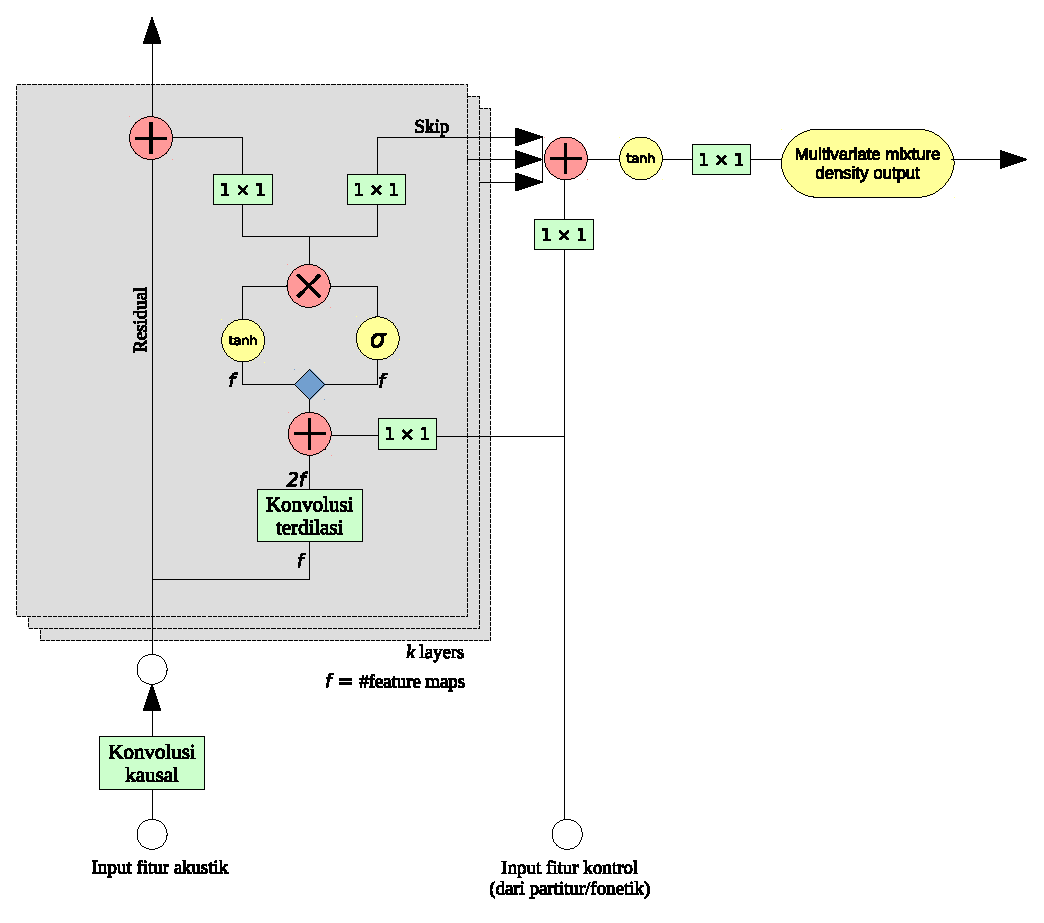
\includegraphics[width=0.8\textwidth]{resources/network-architecture-bonada.eps}
    \caption{Arsitektur jaringan syaraf tiruan modifikasi WaveNet yang digunakan pada sintesis neural parametrik untuk nyanyian\parencite{bonada2017singing}}\label{fig-network-architecture-bonada}
\end{figure}

Model ini menerima masukan fitur akustik dengan konvolusi kausal terdilasi \parencite{Oord2016WaveNetAG}, yang terlihat pada gambar \ref{fig-dilated-cnn}. Dengan demikian, model mampu mempertimbangkan keluaran-keluaran sebelumnya untuk memprediksi fitur akustik pada \textit{frame} selanjutnya. Medan reseptif konteks temporal dari jaringan syaraf tiruan ini, dengan konfigurasi pada riset \citet{bonada2017singing}, mencapai 100ms.

\begin{figure}[h]
    \centering
    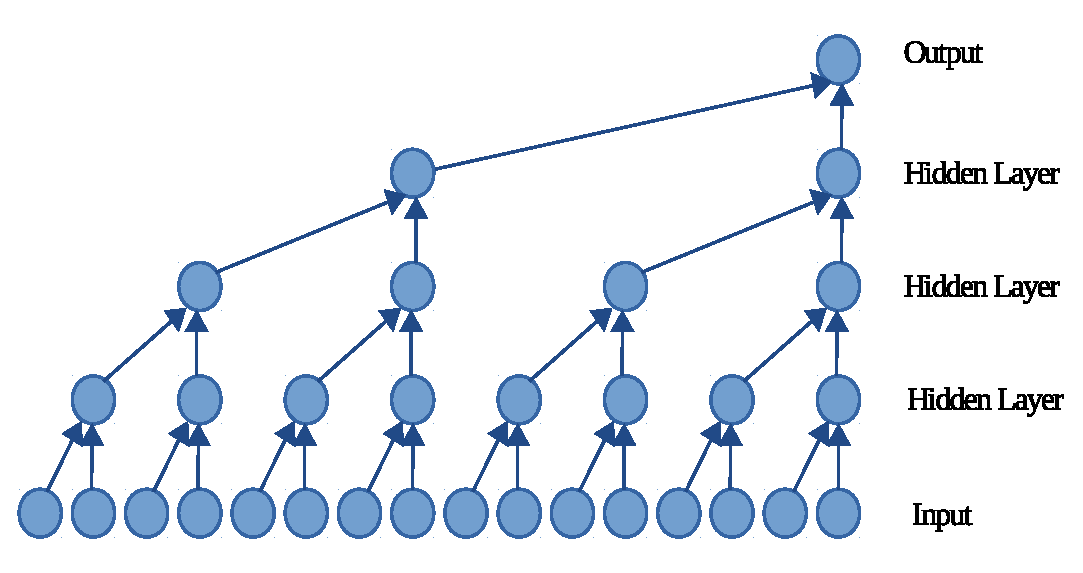
\includegraphics[width=0.8\textwidth]{resources/dilated-cnn.eps}
    \caption{Visualisasi tumpukan lapisan-lapisan konvolusi kausal terdilasi \parencite{Oord2016WaveNetAG}}\label{fig-dilated-cnn}
\end{figure}

Fitur akustik yang telah dilakukan konvolusi kausal terdilasi digabungkan dengan input fitur kontrol dari partitur dan fonetik. Setelah itu, unit aktivasi yang digunakan adalah unit aktivasi bergerbang \parencite{Oord2016ConditionalIG}. Dengan demikian, fungsi aktivasi yang diterapkan kepada masukan gabungan fitur-fitur akustik dan fitur-fitur kontrol menjadi:

\begin{equation}
    \mathbf{z} = tanh(W_{f,k}*\mathbf{x}+V^T_{f,k}\mathbf{h})\odot\sigma(W_{g,k}*\mathbf{x}+V^T_{f,k}\mathbf{h})
\end{equation}\label{eq-gated-activation}

dengan $*$ menunjukkan operator konvolusi, $\odot$ menunjukkan operasi perkalian tiap-elemen, $\sigma$ merupakan fungsi sigmoid, $k$ indeks lapisan, $f$ dan $g$ merupakan filter dan gerbang, $W$ dan $V$ adalah bobot konvolusi untuk masukan fitur akustik dan fitur kontrol yang dapat dipelajari.

Dari satu lapisan ke lapisan lain, diberikan koneksi residual. Serta, dari tiap lapisan, terdapat koneksi skip menuju lapisan output. Dengan cara ini, dapat dilatih jaringan syaraf tiruan yang memiliki lebih banyak lapisan. \parencite{He2016DeepRL}

Pada lapisan output, output tiap lapisan kembali dijumlahkan dengan masukan kontrol. Setelah itu, kembali dikenakan fungsi $tanh$\parencite{bonada2017singing}. Berbeda dengan WaveNet \parencite{Oord2016WaveNetAG} yang menggunakan distribusi keluaran SoftMax, pada teknik neural parametrik digunakan distribusi keluaran \textit{multivariate mixture density}. \textit{Mixture density} yang digunakan adalah Constrained Gaussian Mixture dengan $K=4$ Gaussian: \parencite{bonada2017singing}

\begin{equation}
    p(x) = \sum\limits_{k=0}^{K-1}w_k\mathcal{N}(x;\mu_k,\sigma_k^2)
\end{equation}\label{eq-gated-activation}

Dengan parameter-parameter $w_k$, $\mu_k$, $\sigma_k$ untuk $k=0,1,...,K-1$ dihitung dari empat parameter bebas: $\xi$, skala $\omega$, kemencengan $\alpha$, dan bentuk $\beta$. Bila jaringan memprediksi empat keluaran dengan aktivasi linear, $a_0$, $a_1$, $a_2$, $a_3$, parameter bebas ini diperoleh dengan cara sebagai berikut: \parencite{bonada2017singing}

\begin{equation}
    \xi = 2 sigm(a_0)-1; range[-1,1]
\end{equation}
\begin{equation}
    \omega = \dfrac{2}{255}e^{4sigm(a_1)}; range[\dfrac{2}{255}, \dfrac{2 e^4}{255}]
\end{equation}
\begin{equation}
    \alpha = 2 sigm(a_2)-1; range[-1,1]
\end{equation}
\begin{equation}
    \beta = 2 sigm(a_3); range[0,2]
\end{equation}

Kemudian, parameter-parameter Gaussian $w_k$, $\mu_k$, dan $\sigma_k$ dihitung sebagai berikut:\parencite{bonada2017singing}
\begin{equation}
    \sigma_k = \omega e^{(|\alpha|\gamma_s-1)k|}
\end{equation}
\begin{equation}
    \mu_k = \xi + \sum\limits_{i=0}^{k-1}\sigma_k\gamma_u\alpha
\end{equation}
\begin{equation}
    w_k = \dfrac{\alpha^{2k}\beta{k}\gamma_w^k}{\Sigma_{j=0}{K-1}\alpha^{2i}\beta{i}\gamma_w^i}
\end{equation}

dengan konstanta $\gamma_u$, $\gamma_s$, dan $\gamma_y$ di-$tune$ secara manual.